\documentclass{article}
\usepackage{graphicx} % Required for inserting images
\usepackage{float}
\usepackage{natbib}

\title{MLB Pitcher Injuries and Contributing Factors}
\author{Ajay Natarajan - Statistics Major, University of Connecticut}
\date{October 30, 2023}

\begin{document}

\maketitle

\begin{abstract}
Analytics have become prominent in usage in professional sports within the last two decades. One of the sports that has seen the most advancement within the field is baseball. However, there are various areas within the game of baseball that have had limited research and which are contributing to major inefficiencies at the professional level. A prominent one of these is injuries, particularly to pitchers. This paper will attempt to use available historical injury data as well as existing player and performance data to find significant factors contributing to pitcher injury, and lead insights on how these can be improved.
\end{abstract}

\section{Introduction}
Statistical analysis in sports has been a burgeoning field over the past few decades. In baseball in particular, "analytics" have become especially prominent, with several professional organizations using advanced statistical methods to achieve success and gain a competitive edge. In baseball, one area where it is commonly used is on the side of pitching, enabling pitchers to optimize spin rate, grip, movement, and deception. However, an area with relatively limited study is pitcher injuries. Pitchers are at a relatively high risk of injury, and it has become a growing issue through recent years. This leads to inefficiencies in contract utilization and overall performance for teams, and to lack of career growth for players. 

My research will try to create:
\begin{enumerate}
\item An analysis of the impact of certain on-field factors into the time missed due to pitcher injury. 
\item An analysis of how much time each injury caused the pitcher to miss. As a result, my research inquiries will consist of the following:
\end{enumerate}
\begin{itemize}
  \item Do certain pitcher/performance characteristics cause increased days lost from injury overall?
  \item Can certain pitcher/performance characteristics be used to predict likelihood of player injury, and how well would it do so?
\end{itemize}

\section{Data}
The injury data being utilized in this paper is sourced from two main sources: Fangraphs Roster Report, and Spotrac Injured Reserve Tracker. From these sources, I was able to build an excel database of player injuries. This research utilizes data from 2022 in order to build a recent dataset to work with for pitcher injury data. This creates a sample of 507 different pitcher injuries from Major League pitchers across the season. I cleaned and sorted this data, adding calculations such as total days missed. Added to this database are statistics for each of the pitchers on the list, including fastball velocity, slider velocity, curveball velocity, Earned Run Average, and several other common baseball statistics. I also removed pitchers from the database that did not pitch during the 2022 season, as they had no data to rely on. The dataset contains continuous variables for the independent variables: fastball velocity, slider velocity, curveball velocity, Earned Run Average (ERA), innings pitched (IP), Stuff+ (a measure of the quality of the pitcher's overall repertoire), and strikeouts per nine innings (K/9). 

Below, I have inputted a histogram of total days missed per injury. This illustrates the distribution of days missed due to injury, and shows that there are vastly more shorter-term injuries than there are longer-term ones, with the frequency of longer-term injuries being less as the time missed increases.

\begin{figure}[H]
  \centering
  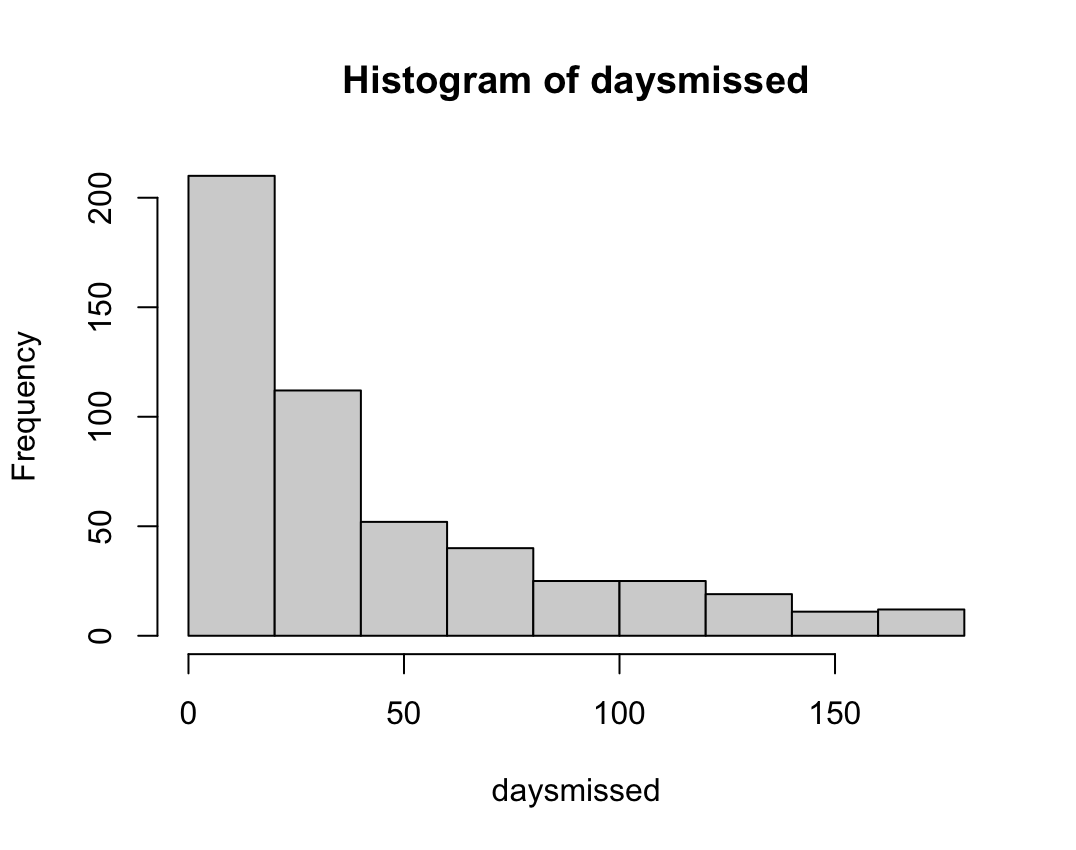
\includegraphics[scale=0.25]{histdaysmissed.png}
  \caption{Days Missed from Injury in 2022}
  \label{fig:Fig1}
\end{figure}

\section{Methods}

Below, I will summarize my methods by several sections, including data preparation and the utilized models and methods to analyze the dataset.

\subsection{Data Preparation}

There were several aspects of the initial dataset that I needed to prepare in order to render it usable for this analysis. 

For one, the initial dataset contained solely injury data from 2022 from all players. I needed to sort this data to exclude position players, since my focus is solely on pitcher injuries. Additionally, the initial dataset did not contain any other of the relevant continuous independent variables, as those were in a different section of Fangraphs. As a result, in preparation of the dataset, I needed to utilize the VLookup command in Excel in order to import the continuous variables to make a utilizable database. Finally, I needed to edit out players who did not throw a pitch in 2022 but were still listed on the injury report, since there is no relevant continuous variable data for each of those players. 

\subsection{Research Questions}

There are several research questions that I am aiming to test. I list them below:

\begin{enumerate}
  \def\labelenumi{\arabic{enumi}.}
  \item
    Is the velocity of fastballs significant on the time lost due to pitcher injuries?
  \item
    Is the velocity of sliders significant on the time lost due to pitcher injuries?
  \item
    Is the velocity of curveballs significant on the time lost due to pitcher injuries?
  \item
    Is the quality of a pitchers repertoire (via Stuff+) significant on the time lost due to pitcher injuries?
  \item
    Is the effectiveness of pitchers (via ERA) significant on the time lost due to pitcher injuries?
  \item
    Is the rate of strikeouts significant on the time lost due to pitcher injuries?
  \item
    Is the overall volume of innings pitched significant on the time lost due to pitcher injuries?
\end{enumerate}

\subsection{Analysis Methods}
For each of the above research questions, I conduct statistical analysis utilizing R. These are tested by using a standard Pearson correlation and a standard linear regression for each question (ie fastball velocity vs days missed). This will use a one-sided T-test to test whether each factor increases the risk of injury. 

Utilizing the levels of significance, we can later focus on certain independent variables that are more significant than others as variables that are especially relevant to the results.

\section{Results}

Using a linear regression model, a table was generated showing the summary of the model results. From this table, we can derive many results.

Here, we can see that the estimated intercept along the model's fit is that a baseline injured pitcher would miss 60.0408 games, with a standard error of 16.6573 games. 

Looking through the continuous variables, we can see some trends. For fastball velocity, the p-value indicates that it is not quite significant, with a p-value above the 0.05 baseline. For its fitted coefficient, it shows that it increases days missed due to injury by 0.1204 for every one mph increase in velocity. For curveball velocity, the p-value also indicates it's not significant, with 0.0607 additional days missed due to injury per mph increase. Slider velocity is also shown to be very insignificant, with a high p-value of 0.9413 and a small fitted coefficient of 0.0044 additional days missed.

For non-velocity continuous variables, significance is also tentative. For repertoire quality, there is a relatively high p-value and a -0.0969 additional days missed. For strikeout rate, there is a somewhat high p-value and a 0.8251 additional days missed per additional strikeout per nine innings. For pitcher performance, there is a somewhat high p-value and a -0.8660 additional days missed per 1 point increase in ERA. For innings pitched, there is an extremely low p-value of 0.000 and a -0.3969 additional days missed.

% latex table generated in R 4.1.3 by xtable 1.8-4 package
% Mon Nov 13 20:41:53 2023
\begin{table}[ht]
\centering
\begin{tabular}{rrrrr}
  \hline
 & Estimate & Std. Error & t value & Pr($>$$|$t$|$) \\ 
  \hline
(Intercept) & 60.0408 & 16.6573 & 3.60 & 0.0003 \\ 
  fastballvelo & 0.1204 & 0.0836 & 1.44 & 0.1505 \\ 
  slidervelo & 0.0044 & 0.0602 & 0.07 & 0.9413 \\ 
  curvevelo & 0.0607 & 0.0469 & 1.29 & 0.1965 \\ 
  stuffplus & -0.0969 & 0.1627 & -0.60 & 0.5518 \\ 
  Kper9 & 0.8251 & 0.8992 & 0.92 & 0.3593 \\ 
  ERA & -0.8660 & 0.8171 & -1.06 & 0.2897 \\ 
  IP & -0.3969 & 0.0411 & -9.65 & 0.0000 \\ 
   \hline
\end{tabular}
\caption{Linear Model Summary} 
\label{tab:lm_summary}
\end{table}

Looking through the results, we can see that no one factor is particularly influential on increasing pitcher injury. This suggests that injury risk is either due to poor luck or more likely to a factor outside the scope of this study (such as poor biomechanics, which have been theorized as a likely source of injury, but which I do not have accessible data for). The most significant factors by the p-value appear to be fastball velocity, curveball velocity, and innings pitched. However, questions must be asked with innings pitched, as that likely covariates with days missed, since increasing days missed would remove opportunities in the finite baseball season to increase innings pitched. As for fastball velocity, that has been theorized to increase pitcher injury (ie. Jacob DeGrom, throwing 101-103mph fastballs getting injured more than Logan Webb, throwing 91-93mph fastballs), so the results are unsurprising. Similar logic has been applied to curveball velocity, so that is unsurprising as well. It's interesting that a similar significance does not apply to slider velocity, but a reasoning likely lies in a biomechanical factor.

\section{Discussion}

This study gives valuable insight onto the impact of certain performance factors onto the time missed due to pitcher injury. It shows that most on-field factors are not significant into determining pitcher injury, although some factors approach a level in which further inquiry may be for the best (such as fastball velocity and curveball velocity). The linear regression indicates that the majority of factors (the velocity factors and strikeout rate) increase time missed due to injury as they increase, though some (performance, repertoire quality, and innings pitched) operate in inverse where higher values (worse performance, better repertoire, more innings pitched) lead to better health.

Several limitations of the study should be brought up. As previously acknowledged, there are other theorized areas for pitcher injury that I have not cited in this study due to a lack of available data, such as on biomechanics. Additionally, the innings pitched statistic appears to covariate, and will likely require further re-work in order to find a way to improve its performance. Finally, this does not include velocities of all pitches, merely the three most common. Some other pitch velocities that could be examined are changeups, sinkers, splitters, and cutters. Finally, a major limitation is database size, as this database only spans 2022, which does not account for injuries that may take a season or longer to deal with, such as UCL reconstruction or ACL tears. 

Given these limitations, there are potential future directions for research, especially if there are more accessible sources of data to work with. Publicly available data on biomechanics (such as, say, average release point) could provide a new avenue of research, as could additional theorized data that was not easily accessible, such as pitcher age. Additionally, building the database to contain multiple years worth of data could allow for time-based analyses and potential time series analysis, and could help account for multi-seasonal injuries. 

Overall, I believe this study does a good job analyzing the impact of on-field factors on pitcher injury in a case study of 2022. I do feel like there is room to broaden the experiment, in time, scope, and in terms of injury type. Baseball is a dynamic sport, and there will be continued opportunities to gather data for injury analysis and refine a potential predictive model to illustrate the future landscape of injuries in Major League Baseball.

\bibliographystyle{chicago}
\bibliography{references}

\end{document}
